%% report.tex
%% V1
%% 04/28/2017
%% by Nafisah Islam
%% See:
%% http://www.michaelshell.org/
%% for current contact information.
%%
%% This is a skeleton file demonstrating the use of IEEEtran.cls
%% (requires IEEEtran.cls version 1.7 or later) with an IEEE conference paper.
%%
%% Support sites:
%% http://www.michaelshell.org/tex/ieeetran/
%% http://www.ctan.org/tex-archive/macros/latex/contrib/IEEEtran/
%% and
%% http://www.ieee.org/

%%*************************************************************************
%% Legal Notice:
%% This code is offered as-is without any warranty either expressed or
%% implied; without even the implied warranty of MERCHANTABILITY or
%% FITNESS FOR A PARTICULAR PURPOSE!
%% User assumes all risk.
%% In no event shall IEEE or any contributor to this code be liable for
%% any damages or losses, including, but not limited to, incidental,
%% consequential, or any other damages, resulting from the use or misuse
%% of any information contained here.
%%
%% All comments are the opinions of their respective authors and are not
%% necessarily endorsed by the IEEE.
%%
%% This work is distributed under the LaTeX Project Public License (LPPL)
%% ( http://www.latex-project.org/ ) version 1.3, and may be freely used,
%% distributed and modified. A copy of the LPPL, version 1.3, is included
%% in the base LaTeX documentation of all distributions of LaTeX released
%% 2003/12/01 or later.
%% Retain all contribution notices and credits.
%% ** Modified files should be clearly indicated as such, including  **
%% ** renaming them and changing author support contact information. **
%%
%% File list of work: IEEEtran.cls, IEEEtran_HOWTO.pdf, bare_adv.tex,
%%                    bare_conf.tex, bare_jrnl.tex, bare_jrnl_compsoc.tex
%%*************************************************************************

% *** Authors should verify (and, if needed, correct) their LaTeX system  ***
% *** with the testflow diagnostic prior to trusting their LaTeX platform ***
% *** with production work. IEEE's font choices can trigger bugs that do  ***
% *** not appear when using other class files.                            ***
% The testflow support page is at:
% http://www.michaelshell.org/tex/testflow/



% Note that the a4paper option is mainly intended so that authors in
% countries using A4 can easily print to A4 and see how their papers will
% look in print - the typesetting of the document will not typically be
% affected with changes in paper size (but the bottom and side margins will).
% Use the testflow package mentioned above to verify correct handling of
% both paper sizes by the user's LaTeX system.
%
% Also note that the "draftcls" or "draftclsnofoot", not "draft", option
% should be used if it is desired that the figures are to be displayed in
% draft mode.
%
\documentclass[conference]{IEEEtran}
\usepackage{blindtext, graphicx, algorithmic}

% hacky table stuff
\usepackage{etoolbox}
\makeatletter
\patchcmd{\@makecaption}
{\scshape}
{}
{}
{}
\makeatother

\def\tablename{Table}
% Add the compsoc option for Computer Society conferences.
%
% If IEEEtran.cls has not been installed into the LaTeX system files,
% manually specify the path to it like:
% \documentclass[conference]{../sty/IEEEtran}





% Some very useful LaTeX packages include:
% (uncomment the ones you want to load)


% *** MISC UTILITY PACKAGES ***
%
%\usepackage{ifpdf}
% Heiko Oberdiek's ifpdf.sty is very useful if you need conditional
% compilation based on whether the output is pdf or dvi.
% usage:
% \ifpdf
%   % pdf code
% \else
%   % dvi code
% \fi
% The latest version of ifpdf.sty can be obtained from:
% http://www.ctan.org/tex-archive/macros/latex/contrib/oberdiek/
% Also, note that IEEEtran.cls V1.7 and later provides a builtin
% \ifCLASSINFOpdf conditional that works the same way.
% When switching from latex to pdflatex and vice-versa, the compiler may
% have to be run twice to clear warning/error messages.






% *** CITATION PACKAGES ***
%
%\usepackage{cite}
% cite.sty was written by Donald Arseneau
% V1.6 and later of IEEEtran pre-defines the format of the cite.sty package
% \cite{} output to follow that of IEEE. Loading the cite package will
% result in citation numbers being automatically sorted and properly
% "compressed/ranged". e.g., [1], [9], [2], [7], [5], [6] without using
% cite.sty will become [1], [2], [5]--[7], [9] using cite.sty. cite.sty's
% \cite will automatically add leading space, if needed. Use cite.sty's
% noadjust option (cite.sty V3.8 and later) if you want to turn this off.
% cite.sty is already installed on most LaTeX systems. Be sure and use
% version 4.0 (2003-05-27) and later if using hyperref.sty. cite.sty does
% not currently provide for hyperlinked citations.
% The latest version can be obtained at:
% http://www.ctan.org/tex-archive/macros/latex/contrib/cite/
% The documentation is contained in the cite.sty file itself.






% *** GRAPHICS RELATED PACKAGES ***
%
\ifCLASSINFOpdf
% \usepackage[pdftex]{graphicx}
% declare the path(s) where your graphic files are
% \graphicspath{{../pdf/}{../jpeg/}}
% and their extensions so you won't have to specify these with
% every instance of \includegraphics
% \DeclareGraphicsExtensions{.pdf,.jpeg,.png}
\else
% or other class option (dvipsone, dvipdf, if not using dvips). graphicx
% will default to the driver specified in the system graphics.cfg if no
% driver is specified.
% \usepackage[dvips]{graphicx}
% declare the path(s) where your graphic files are
% \graphicspath{{../eps/}}
% and their extensions so you won't have to specify these with
% every instance of \includegraphics
% \DeclareGraphicsExtensions{.eps}
\fi
% graphicx was written by David Carlisle and Sebastian Rahtz. It is
% required if you want graphics, photos, etc. graphicx.sty is already
% installed on most LaTeX systems. The latest version and documentation can
% be obtained at:
% http://www.ctan.org/tex-archive/macros/latex/required/graphics/
% Another good source of documentation is "Using Imported Graphics in
% LaTeX2e" by Keith Reckdahl which can be found as epslatex.ps or
% epslatex.pdf at: http://www.ctan.org/tex-archive/info/
%
% latex, and pdflatex in dvi mode, support graphics in encapsulated
% postscript (.eps) format. pdflatex in pdf mode supports graphics
% in .pdf, .jpeg, .png and .mps (metapost) formats. Users should ensure
% that all non-photo figures use a vector format (.eps, .pdf, .mps) and
% not a bitmapped formats (.jpeg, .png). IEEE frowns on bitmapped formats
% which can result in "jaggedy"/blurry rendering of lines and letters as
% well as large increases in file sizes.
%
% You can find documentation about the pdfTeX application at:
% http://www.tug.org/applications/pdftex





% *** MATH PACKAGES ***
%
%\usepackage[cmex10]{amsmath}
% A popular package from the American Mathematical Society that provides
% many useful and powerful commands for dealing with mathematics. If using
% it, be sure to load this package with the cmex10 option to ensure that
% only type 1 fonts will utilized at all point sizes. Without this option,
% it is possible that some math symbols, particularly those within
% footnotes, will be rendered in bitmap form which will result in a
% document that can not be IEEE Xplore compliant!
%
% Also, note that the amsmath package sets \interdisplaylinepenalty to 10000
% thus preventing page breaks from occurring within multiline equations. Use:
%\interdisplaylinepenalty=2500
% after loading amsmath to restore such page breaks as IEEEtran.cls normally
% does. amsmath.sty is already installed on most LaTeX systems. The latest
% version and documentation can be obtained at:
% http://www.ctan.org/tex-archive/macros/latex/required/amslatex/math/





% *** SPECIALIZED LIST PACKAGES ***
%
%\usepackage{algorithmic}
% algorithmic.sty was written by Peter Williams and Rogerio Brito.
% This package provides an algorithmic environment fo describing algorithms.
% You can use the algorithmic environment in-text or within a figure
% environment to provide for a floating algorithm. Do NOT use the algorithm
% floating environment provided by algorithm.sty (by the same authors) or
% algorithm2e.sty (by Christophe Fiorio) as IEEE does not use dedicated
% algorithm float types and packages that provide these will not provide
% correct IEEE style captions. The latest version and documentation of
% algorithmic.sty can be obtained at:
% http://www.ctan.org/tex-archive/macros/latex/contrib/algorithms/
% There is also a support site at:
% http://algorithms.berlios.de/index.html
% Also of interest may be the (relatively newer and more customizable)
% algorithmicx.sty package by Szasz Janos:
% http://www.ctan.org/tex-archive/macros/latex/contrib/algorithmicx/




% *** ALIGNMENT PACKAGES ***
%
%\usepackage{array}
% Frank Mittelbach's and David Carlisle's array.sty patches and improves
% the standard LaTeX2e array and tabular environments to provide better
% appearance and additional user controls. As the default LaTeX2e table
% generation code is lacking to the point of almost being broken with
% respect to the quality of the end results, all users are strongly
% advised to use an enhanced (at the very least that provided by array.sty)
% set of table tools. array.sty is already installed on most systems. The
% latest version and documentation can be obtained at:
% http://www.ctan.org/tex-archive/macros/latex/required/tools/


%\usepackage{mdwmath}
%\usepackage{mdwtab}
% Also highly recommended is Mark Wooding's extremely powerful MDW tools,
% especially mdwmath.sty and mdwtab.sty which are used to format equations
% and tables, respectively. The MDWtools set is already installed on most
% LaTeX systems. The lastest version and documentation is available at:
% http://www.ctan.org/tex-archive/macros/latex/contrib/mdwtools/


% IEEEtran contains the IEEEeqnarray family of commands that can be used to
% generate multiline equations as well as matrices, tables, etc., of high
% quality.


%\usepackage{eqparbox}
% Also of notable interest is Scott Pakin's eqparbox package for creating
% (automatically sized) equal width boxes - aka "natural width parboxes".
% Available at:
% http://www.ctan.org/tex-archive/macros/latex/contrib/eqparbox/





% *** SUBFIGURE PACKAGES ***
%\usepackage[tight,footnotesize]{subfigure}
% subfigure.sty was written by Steven Douglas Cochran. This package makes it
% easy to put subfigures in your figures. e.g., "Figure 1a and 1b". For IEEE
% work, it is a good idea to load it with the tight package option to reduce
% the amount of white space around the subfigures. subfigure.sty is already
% installed on most LaTeX systems. The latest version and documentation can
% be obtained at:
% http://www.ctan.org/tex-archive/obsolete/macros/latex/contrib/subfigure/
% subfigure.sty has been superceeded by subfig.sty.



%\usepackage[caption=false]{caption}
%\usepackage[font=footnotesize]{subfig}
% subfig.sty, also written by Steven Douglas Cochran, is the modern
% replacement for subfigure.sty. However, subfig.sty requires and
% automatically loads Axel Sommerfeldt's caption.sty which will override
% IEEEtran.cls handling of captions and this will result in nonIEEE style
% figure/table captions. To prevent this problem, be sure and preload
% caption.sty with its "caption=false" package option. This is will preserve
% IEEEtran.cls handing of captions. Version 1.3 (2005/06/28) and later
% (recommended due to many improvements over 1.2) of subfig.sty supports
% the caption=false option directly:
%\usepackage[caption=false,font=footnotesize]{subfig}
%
% The latest version and documentation can be obtained at:
% http://www.ctan.org/tex-archive/macros/latex/contrib/subfig/
% The latest version and documentation of caption.sty can be obtained at:
% http://www.ctan.org/tex-archive/macros/latex/contrib/caption/




% *** FLOAT PACKAGES ***
%
%\usepackage{fixltx2e}
% fixltx2e, the successor to the earlier fix2col.sty, was written by
% Frank Mittelbach and David Carlisle. This package corrects a few problems
% in the LaTeX2e kernel, the most notable of which is that in current
% LaTeX2e releases, the ordering of single and double column floats is not
% guaranteed to be preserved. Thus, an unpatched LaTeX2e can allow a
% single column figure to be placed prior to an earlier double column
% figure. The latest version and documentation can be found at:
% http://www.ctan.org/tex-archive/macros/latex/base/



%\usepackage{stfloats}
% stfloats.sty was written by Sigitas Tolusis. This package gives LaTeX2e
% the ability to do double column floats at the bottom of the page as well
% as the top. (e.g., "\begin{figure*}[!b]" is not normally possible in
% LaTeX2e). It also provides a command:
%\fnbelowfloat
% to enable the placement of footnotes below bottom floats (the standard
% LaTeX2e kernel puts them above bottom floats). This is an invasive package
% which rewrites many portions of the LaTeX2e float routines. It may not work
% with other packages that modify the LaTeX2e float routines. The latest
% version and documentation can be obtained at:
% http://www.ctan.org/tex-archive/macros/latex/contrib/sttools/
% Documentation is contained in the stfloats.sty comments as well as in the
% presfull.pdf file. Do not use the stfloats baselinefloat ability as IEEE
% does not allow \baselineskip to stretch. Authors submitting work to the
% IEEE should note that IEEE rarely uses double column equations and
% that authors should try to avoid such use. Do not be tempted to use the
% cuted.sty or midfloat.sty packages (also by Sigitas Tolusis) as IEEE does
% not format its papers in such ways.





% *** PDF, URL AND HYPERLINK PACKAGES ***
%
%\usepackage{url}
% url.sty was written by Donald Arseneau. It provides better support for
% handling and breaking URLs. url.sty is already installed on most LaTeX
% systems. The latest version can be obtained at:
% http://www.ctan.org/tex-archive/macros/latex/contrib/misc/
% Read the url.sty source comments for usage information. Basically,
% \url{my_url_here}.





% *** Do not adjust lengths that control margins, column widths, etc. ***
% *** Do not use packages that alter fonts (such as pslatex).         ***
% There should be no need to do such things with IEEEtran.cls V1.6 and later.
% (Unless specifically asked to do so by the journal or conference you plan
% to submit to, of course. )


% correct bad hyphenation here
%\hyphenation{op-tical net-works semi-conduc-tor}

\usepackage[noadjust]{cite}

\begin{document}
	%
	% paper title
	% can use linebreaks \\ within to get better formatting as desired
	\title{A Hybrid Approach to Improve the Performance of Decision Tree Classifier}


	% author names and affiliations
	% use a multiple column layout for up to three different
	% affiliations
	\author{\IEEEauthorblockN{Trang Ho, Nafisah Islam, Minh Le, John Prewitt, Malcolm Reid Jr.}
		\IEEEauthorblockA{Email: tho25@wisc.edu, nislam@wisc.edu, mle9@wisc.edu, jprewitt@wisc.edu, mreid3@wisc.edu \\
			Computer Sciences\\
			University of Wisconsin - Madison\\
			Madison, Wisconsin 53706\\
			}}

	% conference papers do not typically use \thanks and this command
	% is locked out in conference mode. If really needed, such as for
	% the acknowledgment of grants, issue a \IEEEoverridecommandlockouts
	% after \documentclass

	% for over three affiliations, or if they all won't fit within the width
	% of the page, use this alternative format:
	%
	%\author{\IEEEauthorblockN{Michael Shell\IEEEauthorrefmark{1},
	%Homer Simpson\IEEEauthorrefmark{2},
	%James Kirk\IEEEauthorrefmark{3},
	%Montgomery Scott\IEEEauthorrefmark{3} and
	%Eldon Tyrell\IEEEauthorrefmark{4}}
	%\IEEEauthorblockA{\IEEEauthorrefmark{1}School of Electrical and Computer Engineering\\
	%Georgia Institute of Technology,
	%Atlanta, Georgia 30332--0250\\ Email: see http://www.michaelshell.org/contact.html}
	%\IEEEauthorblockA{\IEEEauthorrefmark{2}Twentieth Century Fox, Springfield, USA\\
	%Email: homer@thesimpsons.com}
	%\IEEEauthorblockA{\IEEEauthorrefmark{3}Starfleet Academy, San Francisco, California 96678-2391\\
	%Telephone: (800) 555--1212, Fax: (888) 555--1212}
	%\IEEEauthorblockA{\IEEEauthorrefmark{4}Tyrell Inc., 123 Replicant Street, Los Angeles, California 90210--4321}}




	% use for special paper notices
	%\IEEEspecialpapernotice{(Invited Paper)}




	% make the title area
	\maketitle


	\begin{abstract}
		In this project, we investigate a potential improvement to decision tree learning by presenting a hybrid classifier that combines decision tree and k-d tree. In this hybrid classifier, the leaf nodes of the decision tree make predictions using k-d tree algorithm instead of the normal majority-based approach. The experimental section shows the results obtained by this new algorithm applied to the MNIST Handwritten Digit Dataset \cite{MNISTDatabase}. ---- TODO: Make conclusion here based on the result compared with other algorithm ----
		%\boldmath
	%	\blindtext[1]
	\end{abstract}
	% IEEEtran.cls defaults to using nonbold math in the Abstract.
	% This preserves the distinction between vectors and scalars. However,
	% if the journal you are submitting to favors bold math in the abstract,
	% then you can use LaTeX's standard command \boldmath at the very start
	% of the abstract to achieve this. Many IEEE journals frown on math
	% in the abstract anyway.

	% Note that keywords are not normally used for peerreview papers.
	\begin{IEEEkeywords}
		Classifier Combination, Decision Tree, K-D Tree, Hybrid Classifier, Dimensionality Reduction.
	\end{IEEEkeywords}


	% For peer review papers, you can put extra information on the cover
	% page as needed:
	% \ifCLASSOPTIONpeerreview
	% \begin{center} \bfseries EDICS Category: 3-BBND \end{center}
	% \fi
	%
	% For peerreview papers, this IEEEtran command inserts a page break and
	% creates the second title. It will be ignored for other modes.
	\IEEEpeerreviewmaketitle

\begin{figure*}[thbp]
	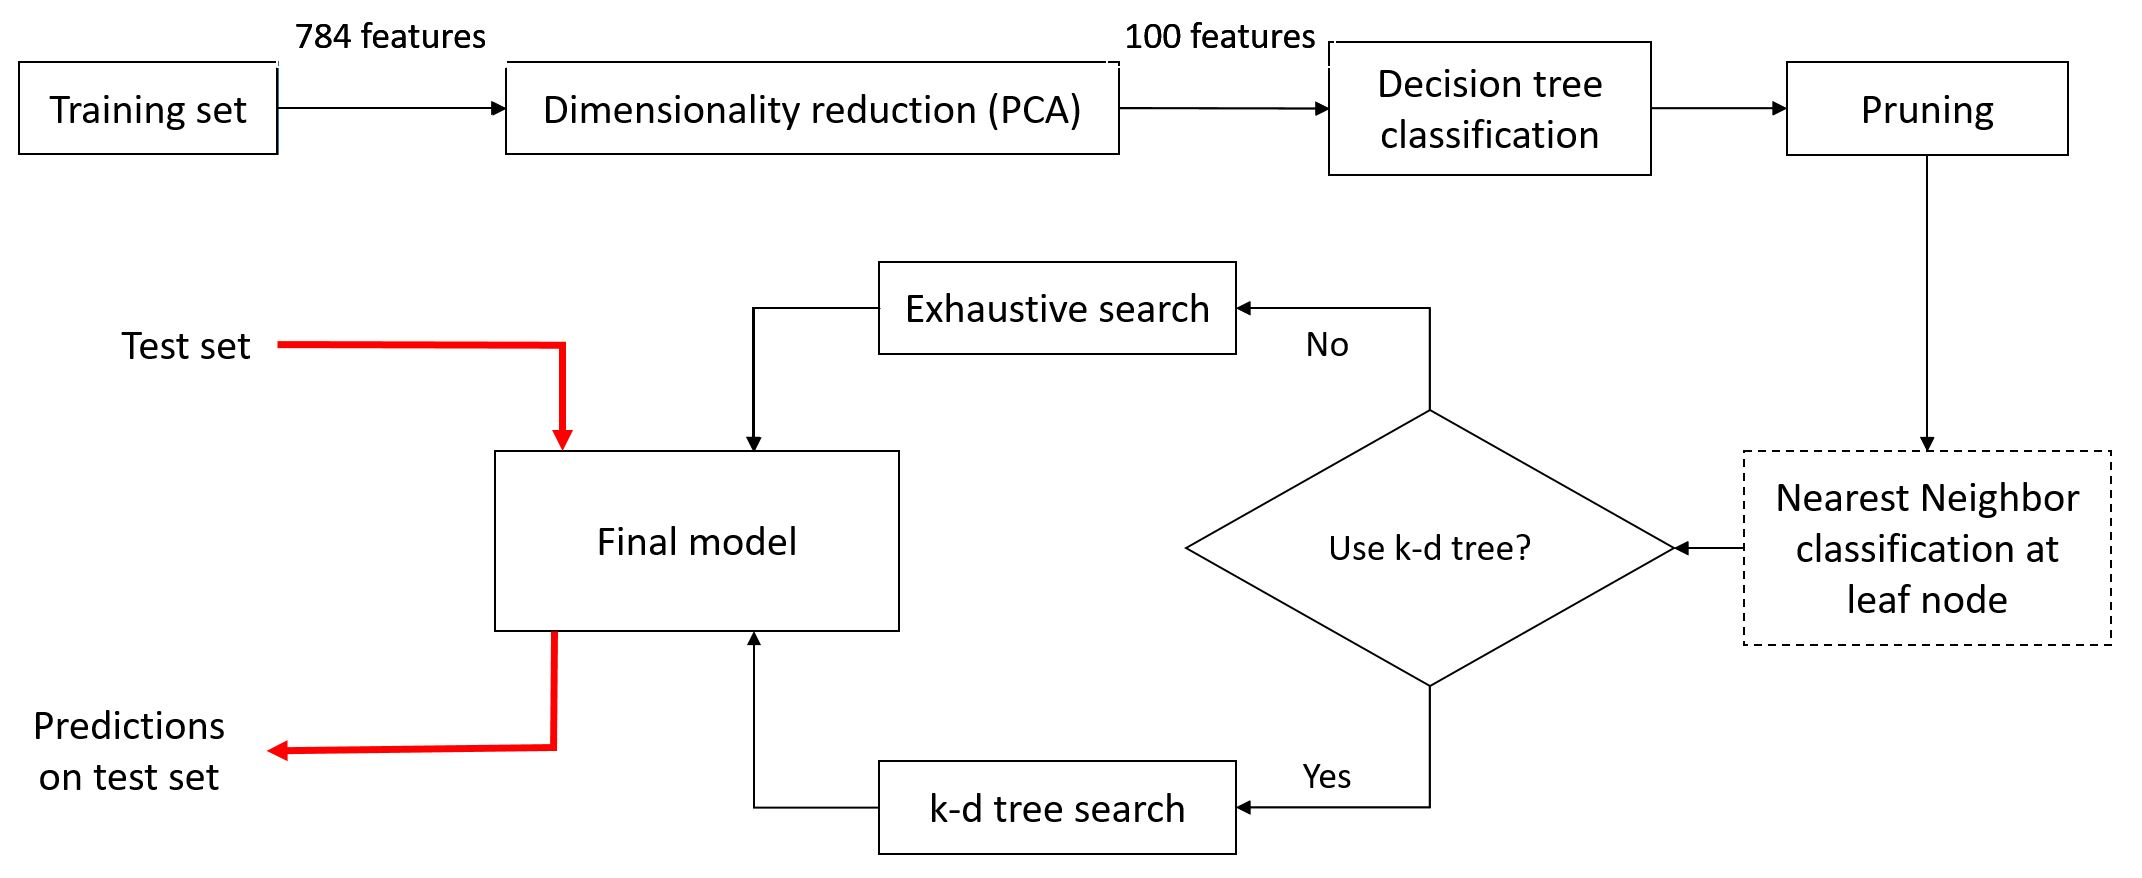
\includegraphics[width=\textwidth]{Figures/workflow.jpg}
	\caption{Algorithm high-level flowchart}
	\label{fig:workflow}
\end{figure*}

\section{Introduction}
Classification is the problem of identifying the category to which observations belong, using information encodes in features of the observation. There are a large number of algorithms that are used for classifying data, across a variety of domains.  We treat these algorithms as being divided into two broad groups: lazy learning algorithms and eager learning algorithms.

  Lazy learning is a form of supervised learning where - during the learning phase, the training examples are simply stored [].  Later, during testing, the testing examples are compared to these training examples using some sort of similarity measure.  There are several instance-based lazy learning algorithms. One of the best known is k-Nearest Neighbor (k-NN) []. During the learning phase, k-NN memorizes training examples. During the classification phase, k-NN uses a similarity measure (such as (squared) Euclidean distance or Hamming distance) to determine the k nearest training examples to a given testing example.  The predicted classification for the testing example is simply whichever label is held by a plurality of the k nearest training examples.  Unfortunately, while lazy learners are very fast during the learning phase, they are much slower during the classification phase, though approaches such as k-d trees sometimes ameliorate this disadvantage.
  
   In contrast with lazy learning we have the eager learning approach, a form of supervised learning in which there is a learning module, a classification module, and a model. Eager learning algorithms invest most of their effort in the learning phase rather than simply "memorizing" the training data like algorithms such as k-NN. Classification of new instances is usually done by the application of a set of rules encoded in the model. Decision tree learning is a widely used approach to this sort of learning. Standard decision trees work by encoding single-feature tests within the interior nodes of the tree and plurality-based predictions at the leaves [].  Decision tree structures are usually learned using information gain as a greedy heuristic [].
   
  Knowing that hybrid classification approaches often work well in practice [], we decided to investigate whether decision trees could be combined with the k-Nearest Neighbors approach.  Rather than working with the entire training set, we could generate k-NN implementations that use only a subset of training data, associated with a leaf node of the decision tree.

  In our hybrid approach, we learn a decision tree using the standard C4.5 algorithm and then associate with each leaf node a subset of the training data that passes the tests to reach that leaf node and a k-d implementation of k-NN learned on that subset. To assess the performance of our hybrid classifier relative to the standard decision tree, we downloaded the MNIST Handwritten Digit Dataset \cite{MNISTDatabase} and used it to generate training, tuning, and testing examples for our algorithm.

\section{Related Work}
Quinlan proposed C4.5 as an improvement to ID3 (cite original C4.5 work). Later, Quinlan further improved C4.5 by changing how the algorithm handles continuous features (cite - improved use of cts attributes). Quinlan proposed C4.5 as an improvement to ID3 \cite{quinlan2014c4}. Though we implemented the original version of C4.5, this is relevant to our work (and a potential improvement to be made in future work) because we used Principal Components Analysis to perform dimensionality reduction.  While the original pixel values were integers in the range 0 to 255, PCA resulted in new features with floating-point values.

Much work has looked at ensemble methods, in which multiple learning algorithms are used to make predictions. We will now provide a brief review of previous work that has used $k$-NN, decision trees, or both in an ensemble method. Todorovski et al. trained several different classifiers on their training set and then used meta decision trees, which are decision trees that, instead of making a prediction at the leaf nodes, decide which base-level classifier to use to make the prediction \cite{todorovski2003combining}. They demonstrated that this stacking approach performs better than using standard decision trees.
Fathi et al. combine $k$-nearest neighbor and decision tree in two ways \cite{FathiMazinani}. In Replacement Based Decisions, they train a decision tree and then convert decisions into vectors of binary decision-features. These vectors are then used to train $k$-NN. In Adding Based Replacement, they add these vectors to the original feature set. They find that both variants improve performance on their intrusion detection system datasets.
Gimenez et al. combine logistic rogression and $k$-NN, using the weights from regression to do a weighted $k$-NN \cite{campillo2013improving}. They find improved performance of this ensemble approach over standard $k$-NN and standard logistic regression. Finally, Martinez-Otzeta et al. preprocess their dataset with nearest neighbor, boosting their training set by duplicating incorrectly classified instances and then use ID3 to create a decision tree \cite{martinezk}. They again find that this ensemble approach performs better than decision trees trained on the unboosted data. 

\section{Dataset}
	Dataset that we used is MNIST database of handwritten digits. This dataset has pixel values (integers from 0 to 255) for 60,000 training examples. The MNIST database contains a separate testing set of 10,000 examples.
\section{Methods}
	\subsection{Algorithms and Combining Methods}
		In our hybrid approach, we combine the decision tree algorithm with a nearest neighbor algorithm (k-d tree or exhaustive search). Figure \ref{fig:workflow} shows the flowchart of the approach over the MNIST dataset. 
		
		First of all, since the number of features in MNIST dataset is too big (784 features), to reduce the training time, we apply principal component analysis (PCA) to the training set to reduce the number of features to 100. Then the training data is input to the decision tree algorithm to obtain a classification tree. After that the tree is pruned, and at each of the leaf nodes, we build a nearest neighbor model to make predictions instead of using the normal majority-approach. The following sections will give more details about Decision Tree and Nearest Neighbor.
		
	\subsection{Decision Tree}
	\subsection{Nearest Neighbor}
		\subsubsection{K-D Tree}
		\subsubsection{Exhaustive Search}


\section{Results}
Our code was written in Python 2.7. When doing time comparisons, we ran the code on a machine with the following specifications: Windows 10 64-bit, Intel 5820k CPU, 32GB memory.

Before running the model on the test data set, we did a speed test between the two versions of Nearest Neighbors, $k$-d tree and exhaustive search, and even though we had a relatively large number of features (100), the $k$-d tree version performed slightly better the exhaustive search. We then decided to use the $k$-d tree version of Nearest Neighbor. 

After running our hybrid decision tree algorithm over the various settings of training, tuning, and testing sets, we generate learning curves to compare the performance of standard decision trees (in which a leaf's associated prediction is based on a plurality of the subset of training data at that leaf) and our hybrid trees.  In Figure \ref{fig:learn_curve}, we can see that the performance of standard trees actually fell off with increased training set size, which provides evidence of overfitting. The hybrid trees, in contrast, showed great improvements in accuracy relative to the standard trees, with the margin increasing for larger training and tuning sets.

\begin{figure}
	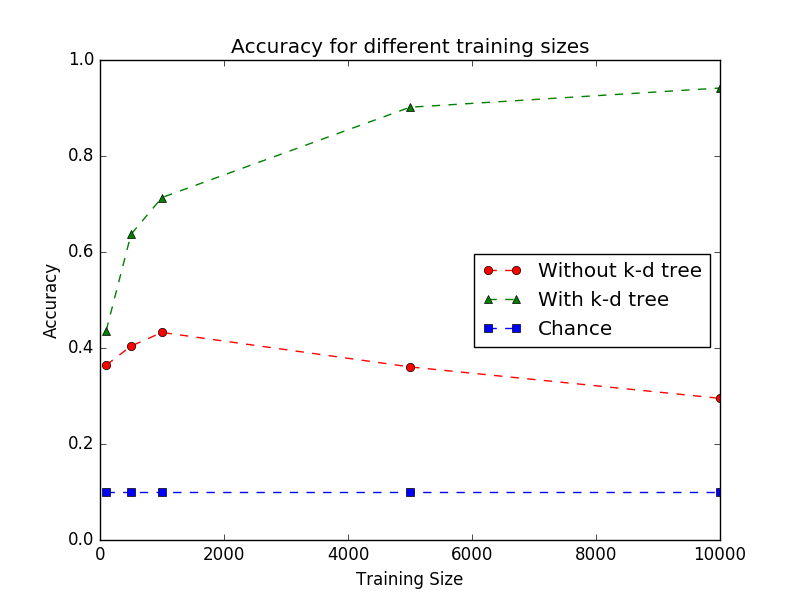
\includegraphics[width=\linewidth]{Figures/learning_curve.png}
	\caption{Learning curve for standard decision trees and hybrid trees with k-d trees.  Note that the chance line assumes a uniform distribution of the 10 handwritten digits.}
	\label{fig:learn_curve}
\end{figure}

To assess the classifier's performance for each handwritten digit, we used the predictions from the setting with 10000 training examples (1000 tuning examples and 10000 testing) to generate a confusion matrix and calculate the values of precision and recall for each digit.  Again, we repeated this for both standard and hybrid decision trees.  Looking at Table \ref{table:no_kd_precision_recall} we can see the digit 2 was never predicted by the standard decision tree.  Other digits, such as 9, exhibit extremely low values of recall. Looking at the confusion matrix in Table \ref{table:no_kd_confusion} we see that the standard decision tree classifier most often predicted the digit 7 for a handwritten 9.  We also have some digits the exhibit unusually low precision coupled with good recall.  For example, the standard decision tree classifier often predicted 1 when presented with examples of other handwritten digits.

Looking at Table \ref{table:with_kd_confusion} and Table \ref{table:with_kd_precision_recall} we can see that the handwritten 2 is actually classifiable (has non-zero precision and recall) by the hybrid classifier.  Additionally, Table \ref{table:with_kd_precision_recall} does not exhibit those sorts of extremely low values of precision and recall.

We also observed an interesting phenomenon with the size and height of the generated decision trees: the size and heights vary widely across the different settings, as shown in \ref{table:dt_sizes}, but there is no monotonic relationship with number of training examples.  For example, both unpruned and pruned trees are smaller for the setting with 10,000 training examples than for the setting with 5,000 training examples (or even 500 or 1,000).

\begin{table}
	\begin{tabular}{r|rrrrrrrrrr}
		&   0 &    1 &   2 &   3 &   4 &   5 &   6 &   7 &   8 &   9 \\
		\hline
		0 & 368 &    3 &   2 &   0 &   1 &   4 &   3 &   2 &   0 &   2 \\
		1 & 517 & 1128 & 444 & 968 &  87 & 742 & 146 & 133 & 866 &  87 \\
		2 &   8 &    0 &   0 &   0 &   0 &   0 &   0 &   0 &   0 &   0 \\
		3 &   0 &    0 &   0 &   1 &   0 &   0 &   0 &   0 &   0 &   0 \\
		4 &   4 &    0 &   1 &   0 &   1 &   0 &   0 &   0 &   3 &   0 \\
		5 &   8 &    0 &   0 &   2 &   0 &   1 &   0 &   0 &   0 &   0 \\
		6 &  42 &    4 & 536 &  21 &  18 &  45 & 561 &   5 &  17 &   3 \\
		7 &  33 &    0 &  49 &  18 & 874 & 100 & 248 & 888 &  86 & 916 \\
		8 &   0 &    0 &   0 &   0 &   1 &   0 &   0 &   0 &   2 &   0 \\
		9 &   0 &    0 &   0 &   0 &   0 &   0 &   0 &   0 &   0 &   1 \\
	\end{tabular}
	\caption{Confusion matrix for standard decision trees.  Note that entries in the top header correspond to the actual labels of the handwritten digits while entries in the left sidebar correspond to the labels predicted by the tree.}
	\label{table:no_kd_confusion}
\end{table}

\begin{table}
	\centering
	\begin{tabular}{rrr}
		Digit &   Precision &      Recall \\
		\hline
		0 &   0.955844  & 0.37551     \\
		1 &   0.220399  & 0.993833    \\
		2 &   0         & 0           \\
		3 &   1         & 0.000990099 \\
		4 &   0.111111  & 0.00101833  \\
		5 &   0.0909091 & 0.00112108  \\
		6 &   0.448083  & 0.585595    \\
		7 &   0.276463  & 0.863813    \\
		8 &   0.666667  & 0.00205339  \\
		9 &   1         & 0.00099108  \\
	\end{tabular}
	\caption{Precision and recall for standard decision trees, for each handwritten digit.}
	\label{table:no_kd_precision_recall}
\end{table}

\begin{table}
	\begin{tabular}{r|rrrrrrrrrr}
		&   0 &    1 &   2 &   3 &   4 &   5 &   6 &   7 &   8 &   9 \\
		\hline
		0 & 940 &    3 &  12 &   0 &   1 &  11 &   8 &   2 &   8 &   7 \\
		1 &   3 & 1125 &   7 &   1 &   9 &   4 &   3 &  22 &   2 &   7 \\
		2 &  10 &    2 & 965 &   9 &   1 &   0 &   0 &   7 &   7 &   2 \\
		3 &   0 &    2 &  12 & 944 &   0 &  25 &   1 &   1 &  33 &   7 \\
		4 &   4 &    0 &   5 &   1 & 909 &   1 &   4 &   4 &   9 &  16 \\
		5 &  12 &    0 &   1 &  22 &   0 & 813 &   2 &   1 &  16 &   3 \\
		6 &   8 &    3 &   3 &   3 &   9 &  19 & 938 &   0 &   7 &   0 \\
		7 &   3 &    0 &  20 &   7 &   7 &   8 &   0 & 975 &   6 &  19 \\
		8 &   0 &    0 &   6 &  12 &   2 &   7 &   2 &   0 & 864 &   5 \\
		9 &   0 &    0 &   1 &  11 &  44 &   4 &   0 &  16 &  22 & 943 \\
	\end{tabular}
	\caption{Confusion matrix for hybrid decision trees.  Note that entries in the top header correspond to the actual labels of the handwritten digits while entries in the left sidebar correspond to the labels predicted by the tree.}
	\label{table:with_kd_confusion}
\end{table}

\begin{table}
	\centering
	\begin{tabular}{rrr}
		Digit &   Precision &   Recall \\
		\hline
		0 &    0.947581 & 0.959184 \\
		1 &    0.950972 & 0.991189 \\
		2 &    0.962114 & 0.935078 \\
		3 &    0.920976 & 0.934653 \\
		4 &    0.95383  & 0.925662 \\
		5 &    0.934483 & 0.911435 \\
		6 &    0.947475 & 0.979123 \\
		7 &    0.933014 & 0.948444 \\
		8 &    0.962138 & 0.887064 \\
		9 &    0.90586  & 0.934589 \\
	\end{tabular}
	\caption{Precision and recall for hybrid decision trees, for each handwritten digit.}
	\label{table:with_kd_precision_recall}
\end{table}

\begin{table}
    \centering
    \begin{tabular}{c|ccccc}
        & 100 & 500 & 1000 & 5000 & 10000 \\
        \hline
        Unpruned & 57 (18) & 153 (46) & 213 (41) & 275 (91) & 91 (17) \\
        Pruned  & 45 (16) & 105 (44)  & 177 (39) & 241 (91) & 65 (16) \\
    \end{tabular}
    \caption{The first number in each table entry is the total number of nodes in unpruned and pruned decision trees built for various numbers of training examples. The second number in parentheses is the height of the tree (that is, the number of nodes from the root to the farthest leaf, inclusive).}
    \label{table:dt_sizes}
\end{table}

\section{Discussion}

We see that our hybrid decision tree algorithm performs better than decision trees with majority labeling. Intuitively, this makes sense as it takes advantage of impure leaves by finding an example similar to the one we are attempting to classify. It is also unsurprising that the hybrid algorithm performs better with more examples. As the decision tree trains on more examples, it is more likely to have seen an example similar to whatever example it is actually trying to classify.

Interestingly, C4.5 performs quite poorly on our data. Possible reasons for this may be noise in the data or overfitting. Also, as Quinlan notes in \cite{quinlan1996improved}, some have noted that C4.5 performs worse in learning settings with continuous attributes than it does in learning settings with discrete attributes. In that same work, Quinlan proposed modifications to C4.5 for improving its performance with continuous attributes. These modifications resulted in smaller decision trees and better accuracy. Future work might examine how the performance of our hybrid approach compares to that of the modified C4.5 learning algorithm.

While our algorithm performs well, it is inefficient. We combine a ``lazy'' learning algorithm with an ``eager'' one to get the worst of both worlds. While $k$-NN learns quickly and takes a long time to classify examples, decision trees take a long time to build and a comparatively short time to classify examples.

Two decisions that we made somewhat arbitrarily but that could be parametrized are the number of components for PCA and the size of the tuning set. We might be able to improve our algorithm by doing a grid search over these parameters. For example, LeCun et al. achieved 96.7\% accuracy on the MNIST dataset after training a classifier with only 40 components after PCA \cite{lecun1998gradient}.

On the systems end, we might look into improving the efficiency of our algorithm. For example, we might try to reduce the number of examples stored in each leaf node by doing edited instance-based learning.
Finally, future work should look into how this algorithm performs in other learning settings and identify in what settings it performs best.

\section{Conclusion}


		%	\blindtext
	% needed in second column of first page if using \IEEEpubid
	%\IEEEpubidadjcol

	% An example of a floating figure using the graphicx package.
	% Note that \label must occur AFTER (or within) \caption.
	% For figures, \caption should occur after the \includegraphics.
	% Note that IEEEtran v1.7 and later has special internal code that
	% is designed to preserve the operation of \label within \caption
	% even when the captionsoff option is in effect. However, because
	% of issues like this, it may be the safest practice to put all your
	% \label just after \caption rather than within \caption{}.
	%
	% Reminder: the "draftcls" or "draftclsnofoot", not "draft", class
	% option should be used if it is desired that the figures are to be
	% displayed while in draft mode.
	%
	%\begin{figure}[!t]
	%\centering
	%\includegraphics[width=2.5in]{myfigure}
	% where an .eps filename suffix will be assumed under latex,
	% and a .pdf suffix will be assumed for pdflatex; or what has been declared
	% via \DeclareGraphicsExtensions.
	%\caption{Simulation Results}
	%\label{fig_sim}
	%\end{figure}

	% Note that IEEE typically puts floats only at the top, even when this
	% results in a large percentage of a column being occupied by floats.


	% An example of a double column floating figure using two subfigures.
	% (The subfig.sty package must be loaded for this to work.)
	% The subfigure \label commands are set within each subfloat command, the
	% \label for the overall figure must come after \caption.
	% \hfil must be used as a separator to get equal spacing.
	% The subfigure.sty package works much the same way, except \subfigure is
	% used instead of \subfloat.
	%
	%\begin{figure*}[!t]
	%\centerline{\subfloat[Case I]\includegraphics[width=2.5in]{subfigcase1}%
	%\label{fig_first_case}}
	%\hfil
	%\subfloat[Case II]{\includegraphics[width=2.5in]{subfigcase2}%
	%\label{fig_second_case}}}
	%\caption{Simulation results}
	%\label{fig_sim}
	%\end{figure*}
	%
	% Note that often IEEE papers with subfigures do not employ subfigure
	% captions (using the optional argument to \subfloat), but instead will
	% reference/describe all of them (a), (b), etc., within the main caption.


	% An example of a floating table. Note that, for IEEE style tables, the
	% \caption command should come BEFORE the table. Table text will default to
	% \footnotesize as IEEE normally uses this smaller font for tables.
	% The \label must come after \caption as always.
	%
	%\begin{table}[!t]
	%% increase table row spacing, adjust to taste
	%\renewcommand{\arraystretch}{1.3}
	% if using array.sty, it might be a good idea to tweak the value of
	% \extrarowheight as needed to properly center the text within the cells
	%\caption{An Example of a Table}
	%\label{table_example}
	%\centering
	%% Some packages, such as MDW tools, offer better commands for making tables
	%% than the plain LaTeX2e tabular which is used here.
	%\begin{tabular}{|c||c|}
	%\hline
	%One & Two\\
	%\hline
	%Three & Four\\
	%\hline
	%\end{tabular}
	%\end{table}


	% Note that IEEE does not put floats in the very first column - or typically
	% anywhere on the first page for that matter. Also, in-text middle ("here")
	% positioning is not used. Most IEEE journals use top floats exclusively.
	% Note that, LaTeX2e, unlike IEEE journals, places footnotes above bottom
	% floats. This can be corrected via the \fnbelowfloat command of the
	% stfloats package.



	% if have a single appendix:
	%\appendix[Proof of the Zonklar Equations]
	% or
	%\appendix  % for no appendix heading
	% do not use \section anymore after \appendix, only \section*
	% is possibly needed

	% use appendices with more than one appendix
	% then use \section to start each appendix
	% you must declare a \section before using any
	% \subsection or using \label (\appendices by itself
	% starts a section numbered zero.)
	%

	% use section* for acknowledgement
	\section*{Acknowledgments}


	The authors would like to thank Professor David Page for his advice and feedback.


	% Can use something like this to put references on a page
	% by themselves when using endfloat and the captionsoff option.
	\ifCLASSOPTIONcaptionsoff
	\newpage
	\fi



	% trigger a \newpage just before the given reference
	% number - used to balance the columns on the last page
	% adjust value as needed - may need to be readjusted if
	% the document is modified later
	%\IEEEtriggeratref{8}
	% The "triggered" command can be changed if desired:
	%\IEEEtriggercmd{\enlargethispage{-5in}}

	% references section

	% can use a bibliography generated by BibTeX as a .bbl file
	% BibTeX documentation can be easily obtained at:
	% http://www.ctan.org/tex-archive/biblio/bibtex/contrib/doc/
	% The IEEEtran BibTeX style support page is at:
	% http://www.michaelshell.org/tex/ieeetran/bibtex/
	%\bibliographystyle{IEEEtran}
	% argument is your BibTeX string definitions and bibliography database(s)
	%\bibliography{IEEEabrv,../bib/paper}
	%
	% <OR> manually copy in the resultant .bbl file
	% set second argument of \begin to the number of references
	% (used to reserve space for the reference number labels box)

	\bibliographystyle{IEEEtran}
	\bibliography{references}

	% biography section
	%
	% If you have an EPS/PDF photo (graphicx package needed) extra braces are
	% needed around the contents of the optional argument to biography to prevent
	% the LaTeX parser from getting confused when it sees the complicated
	% \includegraphics command within an optional argument. (You could create
	% your own custom macro containing the \includegraphics command to make things
	% simpler here.)
	%\begin{biography}[{\includegraphics[width=1in,height=1.25in,clip,keepaspectratio]{mshell}}]{Michael Shell}
	% or if you just want to reserve a space for a photo:

	\begin{IEEEbiography}[{\includegraphics[width=1in,height=1.25in,clip,keepaspectratio]{picture}}]{John Doe}
		\blindtext
	\end{IEEEbiography}

	% You can push biographies down or up by placing
	% a \vfill before or after them. The appropriate
	% use of \vfill depends on what kind of text is
	% on the last page and whether or not the columns
	% are being equalized.

	%\vfill

	% Can be used to pull up biographies so that the bottom of the last one
	% is flush with the other column.
	%\enlargethispage{-5in}




	% that's all folks
\end{document}


